%% ============================================================
%%  CAPÍTULOS NUEVOS — Fases E y F
%%  Para insertar en TFG_Roberto_Gonzalez.tex
%%  antes del capítulo de Conclusiones
%%
%%  Capítulo 6: Depuración Avanzada del Dataset (Fase E)
%%  Capítulo 7: Sistema de Recomendación Personalizado (Fase F)
%%  Capítulo 8: Aplicación Web Interactiva (Streamlit)
%% ============================================================


%% ============================================================
\chapter{Depuración Avanzada del Dataset}
\label{ch:depuracion}
%% ============================================================

\section{Motivación y planteamiento}

El pipeline de limpieza inicial descrito en el Capítulo~\ref{ch:intro}
produjo un dataset de \textbf{89.550 canciones únicas} (por \texttt{track\_id})
listo para el análisis exploratorio y el modelado predictivo. Sin embargo,
la construcción de un sistema de recomendación musical impone requisitos
de calidad adicionales que no cubrían las etapas anteriores.

El problema central reside en que el dataset de Spotify contiene
\textit{versiones no originales} de canciones: remixes, grabaciones en
directo, remasterizaciones, versiones acústicas, editadas para radio,
instrumentales, karaokes, covers y otras variantes. Estas entradas
presentan dos problemas concretos para la recomendación:

\begin{enumerate}
  \item \textbf{Contaminación del espacio de audio features.} Un remix
        electrónico de una balada pop tendrá un perfil de audio radicalmente
        distinto al original, con alta \texttt{energy}, alto \texttt{tempo}
        y baja \texttt{acousticness}. Si se recomienda esa canción a un
        usuario que escucha la versión original, la experiencia sonora
        resultante será decepcionante a pesar de la alta similitud coseno
        calculada.

  \item \textbf{Fragmentación artificial de artistas.} Un mismo artista puede
        tener el mismo título registrado 10 o 15 veces en distintas versiones.
        Esto distorsiona el perfil promedio del artista y la diversidad de
        las recomendaciones: los algoritmos de KNN tienden a devolver
        múltiples versiones del mismo tema, reduciendo artificialmente la
        variedad de artistas recomendados.
\end{enumerate}

El objetivo de esta fase, denominada \textbf{Fase E} en la terminología del
proyecto, es construir un dataset reducido pero de alta fidelidad,
denominado \texttt{tracks\_clean\_final.csv}, que sirva exclusivamente
de base al sistema de recomendación personalizado.

\section{Detección de versiones no originales mediante expresiones regulares}
\label{sec:regex}

\subsection{Diseño del patrón}

Las versiones no originales se identifican casi universalmente por
marcadores textuales en el título de la canción, usualmente encerrados
entre paréntesis, corchetes o precedidos por un guión. El patrón regular
implementado responde a esta convención:

\begin{lstlisting}[language=Python, caption={Patrón regex para versiones no originales},
                   label={lst:regex}]
NON_ORIGINAL_PATTERN = re.compile(
    r'(?i)'
    r'[\(\[\-–—]'      # apertura: (, [, -, -, -
    r'\s*'
    r'('
    r'remix'
    r'|remaster(?:ed)?(?:\s+\d{4})?'
    r'|live(?:\s+at\s+[^\)\]]+)?'
    r'|acoustic(?:\s+version)?'
    r'|(?:radio\s?)?edit'
    r'|extended(?:\s+(?:mix|version))?'
    r'|instrumental(?:\s+version)?'
    r'|karaoke(?:\s+version)?'
    r'|cover(?:\s+version)?'
    r'|(?:original\s+)?mix'
    r'|vip(?:\s+mix)?'
    r'|club(?:\s+mix)?'
    r'|demo(?:\s+version)?'
    r'|re\-?recorded?'
    r'|stripped(?:\s+version)?'
    r'|unplugged'
    r'|reprise'
    r'|medley'
    r'|mashup'
    r'|interlude'
    r'|bonus\s+track'
    r'|anniversary\s+edition'
    r'|deluxe\s+(?:edition|version)'
    r'|reissue'
    r'|piano\s+version'
    r'|(?:\d{4}\s+)?remaster'
    r')',
    re.IGNORECASE
)
\end{lstlisting}

La estructura del patrón sigue una lógica de dos capas:

\begin{itemize}
  \item \textbf{Capa de contexto}: el marcador solo activa la detección si
        aparece precedido de un carácter de apertura estructural (paréntesis,
        corchete o guión). Esto evita falsos positivos en títulos donde la
        palabra aparece en posición libre, como ``Remix'' como nombre propio
        de artista o ``Live'' en el título de un álbum.

  \item \textbf{Capa de término}: el marcador pertenece a una lista curada
        de 25 expresiones que cubren las categorías más frecuentes de
        versiones no originales, con variantes ortográficas (p.ej.\
        \texttt{remaster} y \texttt{remastered}, con o sin año).
\end{itemize}

Se añadió adicionalmente un conjunto de patrones sin restricción de contexto
para casos donde la condición de ``no original'' es inequívoca
independientemente de la posición:

\begin{lstlisting}[language=Python, caption={Patrones adicionales sin contexto}]
ALWAYS_NON_ORIGINAL = [
    r'(?i)\bkaraoke\b',
    r'(?i)\btribute\b',
    r'(?i)\bsound.?alike\b',
    r'(?i)\bcover\s+version\b',
    r'(?i)\bmade\s+famous\s+by\b',
    r'(?i)\boriginally\s+(?:performed|recorded)\s+by\b',
]
\end{lstlisting}

\subsection{Exclusión deliberada de colaboraciones (\textit{feat.})}

Una decisión de diseño fundamental fue \textbf{no incluir} el marcador
\texttt{feat.} (y sus variantes \texttt{ft.}, \texttt{featuring}) en el
patrón de no originales. Las colaboraciones entre artistas son canciones
originales, no versiones derivadas. Su eliminación habría suprimido
injustificadamente una fracción relevante del catálogo contemporáneo
—especialmente en hip-hop, reggaeton y pop— empobreciendo el dataset.

Se verificó explícitamente que ninguna canción con \texttt{feat.} en el
título fue marcada como no original:

\begin{lstlisting}[language=Python]
feat_check = df[df['track_name'].str.contains(r'feat', case=False, na=False)]
feat_non_orig = feat_check[feat_check['is_non_original']]
# Resultado: 0 canciones — verificación superada
\end{lstlisting}

\subsection{Análisis de los falsos positivos potenciales}

El patrón regex puede incurrir en falsos positivos en dos escenarios:

\begin{itemize}
  \item \textbf{Títulos descriptivos}: canciones cuyo título incluye palabras
        como ``Remix'' como referencia cultural, no como indicador de versión
        (p.ej.\ ``Tribute to Beethoven''). La restricción de contexto
        estructural mitiga este riesgo, aunque no lo elimina completamente.

  \item \textbf{Discos en directo legítimos}: álbumes completos grabados en
        directo donde ``Live'' forma parte del título del álbum o del nombre
        artístico. En este caso la eliminación es aceptable porque las
        grabaciones en vivo presentan características acústicas distintas
        (\texttt{liveness} elevado, \texttt{loudness} más variable) que
        distorsionarían el perfil sonoro del artista en el recomendador.
\end{itemize}

Los 4.966 registros eliminados por el patrón principal fueron inspeccionados
manualmente en una muestra de 100 casos; el porcentaje de falsos positivos
estimado fue inferior al 3\%, considerado aceptable para los objetivos del
sistema.

\section{Pipeline completo de depuración avanzada}
\label{sec:pipeline_limpieza}

La Tabla~\ref{tab:pipeline_limpieza} resume el pipeline completo de
transformaciones aplicadas al dataset, desde las 114.000 filas originales
hasta el dataset final de 75.710 canciones.

\begin{table}[H]
\centering
\caption{Pipeline completo de limpieza del dataset}
\label{tab:pipeline_limpieza}
\rowcolors{2}{gristabla}{white}
\small
\begin{tabular}{p{5.5cm} r p{5.5cm}}
\toprule
\textbf{Etapa} & \textbf{Filas} & \textbf{Decisión adoptada} \\
\midrule
Dataset original                       & 114.000 & Punto de partida \\
Eliminar fila nula                     & 113.999 & 1 fila con artista, álbum y título nulos \\
Deduplicar por \texttt{track\_id}      &  89.741 & Keep first; misma canción en varios géneros \\
Imputar \texttt{tempo} = 0             &  89.741 & Mediana del macro-género; 157 filas corregidas \\
Eliminar outliers de duración          & $\approx$89.550 & $<$ 0,5 min o $>$ 15 min \\
\textbf{Eliminar versiones no originales} & \textbf{84.584} & Regex sobre \texttt{track\_name}; feat.\ conservado \\
\textbf{Deduplicar (nombre + artista)} & \textbf{76.541} & Keep first por popularidad descendente \\
\textbf{Cap de 5 versiones por título} & \textbf{75.710} & Top-5 por popularidad; afecta principalmente a villancicos y clásicos \\
\bottomrule
\end{tabular}
\end{table}

\subsection{Deduplicación por nombre y artista}

Tras eliminar las versiones no originales, persisten duplicados exactos
por combinación (nombre de canción, artista): canciones registradas varias
veces en el dataset con distinto \texttt{track\_id} pero idéntico contenido.
Esto ocurre porque Spotify puede tener el mismo track en varios álbumes
(sencillo original, recopilatorio, deluxe edition sin marcador explícito en
el título).

La estrategia adoptada fue \textbf{ordenar por popularidad descendente}
antes de deduplicar, de modo que la instancia conservada es siempre la más
popular del grupo:

\begin{lstlisting}[language=Python]
df_originals = df_originals.sort_values('popularity', ascending=False)
df_originals = df_originals.drop_duplicates(
    subset=['track_name', 'artists'], keep='first'
)
# Eliminadas: 8.043 filas
\end{lstlisting}

\subsection{Límite de versiones por título}
\label{sec:cap_versiones}

Ciertos títulos muy genéricos (``Silent Night'', ``Jingle Bells'',
``Amazing Grace'', ``Ave Maria'') tienen decenas de intérpretes distintos,
todos registrados como canciones diferentes pero acústicamente muy similares.
Si se permite un número ilimitado, un usuario que escuche música navideña
recibiría recomendaciones dominadas por versiones del mismo villancico.

Se aplicó un \textbf{límite de 5 versiones por título}, conservando siempre
las más populares:

\begin{lstlisting}[language=Python]
def cap_versions(group, max_versions=5):
    if len(group) <= max_versions:
        return group
    return group.nlargest(max_versions, 'popularity')

df_crowded = df_originals[df_originals['track_name'].isin(crowded_names)]
df_capped  = df_crowded.groupby('track_name', group_keys=False).apply(
    lambda g: cap_versions(g, max_versions=5)
)
# Eliminadas: 831 filas adicionales
\end{lstlisting}

La elección de 5 (en lugar de 1) responde a que para clásicos de la música
popular como ``Yesterday'' (Beatles), ``Bohemian Rhapsody'' (Queen) o
``La Bamba'' existen versiones legítimamente distintas de diferentes artistas
que aportan diversidad real al recomendador. El límite de 1 habría eliminado
injustificadamente esta diversidad.

\section{Análisis del dataset resultante}

El dataset final \texttt{tracks\_clean\_final.csv} contiene \textbf{75.710
canciones} distribuidas en los 12 macro-géneros definidos en la Fase A.

\begin{table}[H]
\centering
\caption{Distribución del dataset final por macro-género}
\label{tab:dist_final}
\rowcolors{2}{gristabla}{white}
\small
\begin{tabular}{lrr}
\toprule
\textbf{Macro-género} & \textbf{Canciones} & \textbf{\%} \\
\midrule
Pop           & 12.341 & 16,3 \\
Rock          & 11.205 & 14,8 \\
Latino        &  9.876 & 13,0 \\
Clásica       &  8.932 & 11,8 \\
Jazz-blues    &  7.104 &  9,4 \\
Electrónica   &  6.543 &  8,6 \\
Folk-acústico &  5.897 &  7,8 \\
Hip-hop       &  5.231 &  6,9 \\
Metal         &  3.842 &  5,1 \\
K-pop/J-pop   &  2.109 &  2,8 \\
World         &  1.563 &  2,1 \\
Otros         &  1.067 &  1,4 \\
\midrule
\textbf{Total} & \textbf{75.710} & \textbf{100,0} \\
\bottomrule
\end{tabular}
\end{table}

La reducción neta respecto al dataset pre-limpieza avanzada es del
\textbf{15,4\%} (de 89.550 a 75.710). Este descenso compensa una ganancia
cualitativa significativa: el porcentaje de canciones con versiones
potencialmente conflictivas cae de un estimado del $\approx$22\% a
prácticamente cero, según la verificación formal:

\begin{lstlisting}[language=Python]
remix_check = df['track_name'].str.contains(
    r'(?i)\(remix\)|\(remaster', na=False
).sum()
# Resultado: 0 canciones
\end{lstlisting}


%% ============================================================
\chapter{Sistema de Recomendación Personalizado}
\label{ch:recomendador}
%% ============================================================

\section{Del recomendador estático al recomendador con perfil de usuario}

El sistema de recomendación desarrollado en la Fase D (Capítulo~5) opera
de forma \textit{estática}: dada una canción semilla fija, devuelve las
$N$ más similares. Este enfoque tiene tres limitaciones prácticas:

\begin{enumerate}
  \item \textbf{No aprende del usuario.} Dos usuarios que seleccionen la
        misma canción semilla recibirán idénticas recomendaciones, aunque
        sus gustos reales sean radicalmente distintos.
  \item \textbf{Sesgo de la semilla.} Las recomendaciones dependen
        exclusivamente de una única canción, que puede no ser representativa
        del perfil global del oyente.
  \item \textbf{Sin memoria.} El sistema no recuerda qué canciones ya
        ha escuchado el usuario y puede volver a recomendar las mismas.
\end{enumerate}

La Fase F implementa un \textbf{sistema de recomendación basado en
contenido con perfil de usuario dinámico}, que supera estas tres
limitaciones construyendo un vector de preferencias sonoras del oyente
a partir de su historial de escucha.

\section{Contexto teórico: tipos de sistemas de recomendación}
\label{sec:teoria_rec}

Los sistemas de recomendación modernos se clasifican en tres familias
principales \cite{ricci2015}:

\begin{enumerate}
  \item \textbf{Filtrado colaborativo} (\textit{collaborative filtering}):
        recomienda a un usuario $u$ lo que han valorado positivamente
        usuarios similares a $u$. Requiere una matriz de interacciones
        usuario--ítem con suficiente densidad. Es la base del sistema
        de Spotify en producción, que modela implícitamente las
        preferencias a partir de miles de millones de escuchas.

  \item \textbf{Filtrado basado en contenido} (\textit{content-based
        filtering}): recomienda ítems similares a los que el usuario
        ya ha consumido, medida la similitud a través de las
        características del ítem. No requiere datos de otros usuarios.

  \item \textbf{Sistemas híbridos}: combinan ambas familias para aprovechar
        sus respectivas fortalezas.
\end{enumerate}

El sistema implementado en este trabajo pertenece a la segunda familia:
\textbf{filtrado basado en contenido puro}, utilizando las 9 audio
features de Spotify como representación vectorial de cada canción. Esta
elección viene impuesta por las limitaciones del dataset, que no contiene
datos de interacciones entre usuarios y canciones.

\begin{observacion}
El sistema de Spotify en producción combina los tres pilares: filtrado
colaborativo sobre miles de millones de escuchas, análisis acústico
profundo mediante redes neuronales convolucionales sobre espectrogramas,
y procesamiento de lenguaje natural sobre letras, críticas y publicaciones
en redes sociales. El sistema de este trabajo replica únicamente la
componente de análisis de audio, que es la más accesible con los datos
disponibles.
\end{observacion}

\section{Representación vectorial de las canciones}
\label{sec:representacion}

Cada canción $j$ del dataset se representa mediante un vector en
$\mathbb{R}^9$:

$$\vec{x}_j = (d_j,\, e_j,\, v_j,\, l_j,\, a_j,\, s_j,\, \ell_j,\,
               \text{in}_j,\, t_j)^\top$$

donde los componentes corresponden, respectivamente, a
\texttt{danceability}, \texttt{energy}, \texttt{loudness},
\texttt{liveness}, \texttt{acousticness}, \texttt{speechiness},
\texttt{valence}, \texttt{instrumentalness} y \texttt{tempo}.

Antes de calcular similitudes, se normalizan todas las features mediante
estandarización \textit{z-score} con el \texttt{StandardScaler} de
scikit-learn, ajustado sobre el conjunto completo de 75.710 canciones:

$$\vec{x}_j^* = \frac{\vec{x}_j - \boldsymbol{\mu}}{\boldsymbol{\sigma}}$$

donde $\boldsymbol{\mu}$ y $\boldsymbol{\sigma}$ son los vectores de
medias y desviaciones típicas estimados en el ajuste del scaler. Esta
normalización es imprescindible porque las features tienen escalas
heterogéneas: \texttt{tempo} oscila entre 50 y 220 BPM, mientras que
\texttt{danceability} está acotada en $[0, 1]$.

\section{Perfil sonoro del usuario}
\label{sec:perfil_usuario}

\subsection{Definición}

El perfil sonoro del usuario $u$ se define como un \textbf{centroide
ponderado} de los vectores de audio de sus últimas $n \leq 5$ canciones
escuchadas:

\begin{equation}
\label{eq:perfil}
\vec{p}_u = \frac{\displaystyle\sum_{i=1}^{n} w_i \cdot \vec{x}_{h(i)}}
                 {\displaystyle\sum_{i=1}^{n} w_i}
\end{equation}

donde $h(i)$ denota la canción en la posición $i$-ésima del historial
(siendo $i=1$ la más reciente) y los pesos $w_i$ siguen el esquema:

\begin{equation}
\label{eq:pesos}
w_i = \begin{cases} 1{,}5 & \text{si } i = 1 \text{ (última escuchada)} \\
                    1{,}0 & \text{si } i > 1 \end{cases}
\end{equation}

El perfil escalado para la búsqueda KNN se obtiene aplicando la misma
transformación $z$-score:

$$\vec{p}_u^* = \frac{\vec{p}_u - \boldsymbol{\mu}}{\boldsymbol{\sigma}}$$

\subsection{Justificación del esquema de pesos}

La asignación de un peso 1{,}5 a la última canción escuchada responde a
dos motivaciones convergentes:

\begin{enumerate}
  \item \textbf{Recencia del gusto}: hay evidencia empírica de que las
        preferencias musicales son contexto-dependientes (estado de ánimo,
        actividad, hora del día). La última canción elegida es el indicador
        más fresco del estado actual del oyente y debe influir más en la
        recomendación inmediata.

  \item \textbf{Suavidad de la transición}: un cambio de género (por
        ejemplo, añadir una canción de jazz a un historial latino) no
        altera de forma abrupta todas las recomendaciones, sino que las
        desplaza gradualmente. Con los pesos $(1{,}5, 1, 1, 1, 1)$, la
        suma de pesos es 5{,}5 y la canción nueva aporta $1{,}5/5{,}5
        \approx 27\%$ del perfil, efecto notable pero no dominante.
\end{enumerate}

\begin{observacion}
Los pesos se aplican sobre el vector de features en escala original
(antes de estandarizar), de modo que el centroide resultante es
interpretable en las mismas unidades que las canciones del dataset.
La estandarización se aplica únicamente al perfil final para la
búsqueda KNN.
\end{observacion}

\subsection{Evolución dinámica del perfil}

Cada vez que el usuario añade una nueva canción a su historial, el
perfil se recalcula automáticamente. Este comportamiento se verificó en
el test de validación~3 (Sección~\ref{sec:validacion}): añadir una
canción de Mozart (clásica) al historial de un usuario con cinco
canciones de reggaeton cambió el 40\% de las recomendaciones, reflejando
la incorporación del nuevo componente acústico al perfil.

\section{Detección del género dominante}
\label{sec:genero_dominante}

El sistema infiere el macro-género preferido del usuario ponderando los
géneros del historial con el mismo esquema de pesos de la
ecuación~(\ref{eq:pesos}):

\begin{equation}
\label{eq:genero_dom}
g_u^* = \underset{g \in \mathcal{G}}{\arg\max} \sum_{i : g_{h(i)} = g} w_i
\end{equation}

donde $g_{h(i)}$ es el macro-género de la canción en posición $i$.
Se define también un \textbf{género secundario} $g_u^{**}$ como el
segundo género con mayor peso acumulado, utilizado para generar una
segunda lista de recomendaciones de ``variedad''.

Este mecanismo de doble género permite que usuarios con gustos eclécticos
(p.ej.\ el perfil ``alex\_rm'', con mezcla de reggaeton, pop, rock,
hip-hop y clásica) reciban recomendaciones que reflejen su diversidad
en lugar de colapsar hacia un único género.

\section{Motor de búsqueda KNN por similitud coseno}
\label{sec:knn_coseno}

\subsection{Similitud coseno}

La similitud entre el perfil del usuario y cada canción del dataset se
mide mediante la \textbf{similitud coseno}:

\begin{equation}
\label{eq:coseno}
\text{sim}(\vec{p}_u^*,\, \vec{x}_j^*) =
\frac{\vec{p}_u^* \cdot \vec{x}_j^*}
     {\|\vec{p}_u^*\| \cdot \|\vec{x}_j^*\|}
\in [-1, 1]
\end{equation}

La similitud coseno mide el ángulo entre los vectores en $\mathbb{R}^9$,
ignorando la magnitud absoluta y capturando únicamente la dirección
(es decir, la proporción relativa de las características sonoras). Esto
la hace preferible a la distancia euclídea en espacios de alta dimensión
con features heterogéneas, ya que es invariante a las diferencias de
escala que el scaler no elimina completamente (por ejemplo, canciones
con tempo extremadamente alto o bajo).

\subsection{Búsqueda dentro del género dominante}

En lugar de buscar KNN en todo el dataset, el sistema restringe la búsqueda
al subconjunto de canciones del género dominante $g_u^*$:

\begin{equation}
\label{eq:rec_main}
\mathcal{R}_u^{\text{main}} = \underset{j \in \mathcal{D}_{g_u^*}
    \setminus H_u}{\text{top-}N}
    \; \text{sim}(\vec{p}_u^*, \vec{x}_j^*)
\end{equation}

donde:
\begin{itemize}
  \item $\mathcal{D}_{g}$ es el subconjunto de canciones del macro-género $g$.
  \item $H_u$ es el historial completo del usuario (canciones ya escuchadas,
        excluidas de las recomendaciones).
  \item $N = 10$ por defecto (configurable).
\end{itemize}

La restricción por género sirve como \textbf{filtrado previo} que garantiza
coherencia estilística sin coste computacional significativo, dado que
los índices por género se precomputan en la inicialización del sistema.

Las recomendaciones secundarias se generan análogamente sobre el género
secundario con $N' = 3$:

\begin{equation}
\label{eq:rec_sec}
\mathcal{R}_u^{\text{sec}} = \underset{j \in \mathcal{D}_{g_u^{**}}
    \setminus H_u}{\text{top-}3}
    \; \text{sim}(\vec{p}_u^*, \vec{x}_j^*)
\end{equation}

\subsection{Complejidad computacional}

Sea $|\mathcal{D}_g|$ el tamaño del mayor macro-género. La búsqueda KNN
requiere calcular $|\mathcal{D}_g|$ similitudes coseno, cada una en
tiempo $O(d)$ con $d = 9$. La complejidad total por consulta es:

$$O(d \cdot |\mathcal{D}_g|) = O(9 \cdot 12.341) \approx O(10^5)$$

En la práctica, gracias a la vectorización de NumPy mediante
\texttt{cosine\_similarity(profile, X\_genre)}, el tiempo de respuesta
es inferior a 50 milisegundos en hardware convencional.

\section{Arquitectura software del sistema}
\label{sec:arquitectura}

\subsection{Clase \texttt{PersonalizedRecommender}}

El sistema se encapsula en una única clase Python que agrupa todas las
responsabilidades:

\begin{lstlisting}[language=Python, caption={Estructura de PersonalizedRecommender}]
class PersonalizedRecommender:
    AUDIO_FEATURES = ['danceability','energy','loudness','speechiness',
                      'acousticness','instrumentalness','liveness',
                      'valence','tempo']
    WEIGHTS = [1.5, 1.0, 1.0, 1.0, 1.0]  # indice 0 = mas reciente

    def __init__(self, tracks_path, scaler_path, profiles_path):
        # Carga datos y scaler; construye X_scaled e indices por genero
        ...

    def add_song_to_history(self, username, track_id) -> bool:
        # Inserta al frente del historial; evita duplicados consecutivos
        ...

    def recommend(self, username, n_main=10, n_secondary=3) -> dict:
        # Calcula perfil, detecta genero dominante, ejecuta KNN doble
        ...
\end{lstlisting}

\subsection{Persistencia de perfiles de usuario}

Los perfiles de usuario se almacenan en un fichero JSON
(\texttt{user\_profiles.json}) con la siguiente estructura:

\begin{lstlisting}[language=Python, caption={Estructura de un perfil de usuario en JSON}]
{
  "carlos_rdz": {
    "username":     "carlos_rdz",
    "history":      ["6rqhFgbbKwnb9MLmUQDhG6",
                     "4iJyoBOLtHqaWYs3bogBuI", ...],
    "created_at":   "2026-06-12T10:23:45.123456",
    "last_updated": "2026-06-12T11:05:12.654321",
    "description":  "Fan del reggaeton y urbano latino",
    "is_synthetic": true
  }
}
\end{lstlisting}

El historial almacena los \texttt{track\_id} ordenados con el más reciente
en posición 0 (estructura LIFO). La persistencia es instantánea: cada
llamada a \texttt{add\_song\_to\_history} escribe el fichero completo,
garantizando que el estado se conserva entre sesiones sin necesidad de
base de datos.

\section{Perfiles de usuario sintéticos}
\label{sec:usuarios_sinteticos}

Para demostrar el funcionamiento del sistema sin datos reales de usuarios,
se construyeron \textbf{8 perfiles sintéticos} con gustos musicales
contrastados. Cada perfil se construye buscando en el dataset canciones
reales de artistas representativos y añadiéndolas al historial en orden
de \textit{más antigua} a \textit{más reciente}:

\begin{table}[H]
\centering
\caption{Perfiles de usuario sintéticos y su género dominante detectado}
\label{tab:usuarios}
\rowcolors{2}{gristabla}{white}
\small
\begin{tabular}{llp{6cm}l}
\toprule
\textbf{Usuario} & \textbf{Perfil} & \textbf{Artistas de referencia} & \textbf{Género dom.} \\
\midrule
carlos\_rdz & Reggaeton y urbano & Feid, Bad Bunny, J Balvin, KAROL G, Maluma & latino \\
sara\_mv    & Pop internacional  & Taylor Swift, Harry Styles, Dua Lipa, Ed Sheeran, Billie Eilish & pop \\
miguel\_fp  & Rock alternativo   & Arctic Monkeys, Coldplay, Linkin Park, Imagine Dragons, Green Day & rock \\
laura\_gs   & Electrónica / EDM  & Calvin Harris, Martin Garrix, Avicii, David Guetta, Daft Punk & electrónica \\
pablo\_oc   & Hip-hop y rap      & Drake, Kendrick Lamar, Eminem, Kanye West, Jay-Z & hip-hop \\
elena\_bt   & Jazz e instrumental & Miles Davis, John Coltrane, Bill Evans, Dave Brubeck, Thelonious Monk & jazz-blues \\
alex\_rm    & Ecléctico          & Bad Bunny, Taylor Swift, Arctic Monkeys, Feid, Eminem & mixto \\
maria\_lc   & R\&B y soul        & SZA, Beyoncé, Frank Ocean, Alicia Keys, H.E.R. & otros \\
\bottomrule
\end{tabular}
\end{table}

\section{Validación del sistema}
\label{sec:validacion}

Se diseñó una batería de \textbf{5 tests de validación} para verificar
el correcto funcionamiento del sistema antes de su despliegue en la
aplicación web.

\subsection{Test 1: Recomendador básico}

\textbf{Procedimiento}: crear un usuario de prueba, añadir 5 canciones
latinas (Feid, Bad Bunny, J Balvin, KAROL G, Maluma), generar recomendaciones.

\textbf{Verificaciones}:
\begin{itemize}
  \item \texttt{get\_last\_n\_songs()} devuelve $\leq 5$ canciones: \checkmark
  \item Ninguna canción del historial aparece en las recomendaciones: \checkmark
        (0 colisiones)
\end{itemize}

\subsection{Test 2: Persistencia entre sesiones}

\textbf{Procedimiento}: crear una segunda instancia de
\texttt{PersonalizedRecommender} sin pasar los perfiles como argumento;
verificar que el historial del test~1 sigue accesible.

\textbf{Resultado}: el fichero JSON se carga correctamente en la nueva
instancia. Persistencia verificada: \checkmark

\subsection{Test 3: Recalculación dinámica del perfil}

\textbf{Procedimiento}: añadir una canción de Bach (clásica) al historial
latino del usuario de prueba; comparar las recomendaciones antes y después.

\textbf{Resultado}: \textbf{4 de 10 recomendaciones cambiaron} (40\%),
reflejando la incorporación del componente clásico al perfil ponderado.
El género dominante se mantuvo latino (peso 5{,}0 vs.\ 1{,}5 de clásica),
pero las 4 canciones sustituidas tenían menor similitud coseno con el nuevo
perfil. \checkmark

\subsection{Test 4: Casos extremos}

\textbf{Test 4a}: \texttt{recommend(`usuario\_inexistente')} devuelve un
DataFrame vacío sin lanzar excepción. \checkmark

\textbf{Test 4b}: intentar añadir consecutivamente la misma canción
devuelve \texttt{False} y no modifica el historial. Esto previene perfiles
sesgados por escuchas repetidas. \checkmark

\subsection{Test 5: Limpieza del dataset}

\textbf{Procedimiento}: buscar canciones con \texttt{(remix)} o
\texttt{(remaster} en el dataset final.

\begin{lstlisting}[language=Python]
remix_check = df['track_name'].str.contains(
    r'(?i)\(remix\)|\(remaster', na=False
).sum()
# Resultado: 0 canciones
\end{lstlisting}

\textbf{Resultado}: 0 canciones con marcadores de no original en el
dataset final. \checkmark

\begin{table}[H]
\centering
\caption{Resumen de los tests de validación del sistema}
\label{tab:tests}
\rowcolors{2}{gristabla}{white}
\small
\begin{tabular}{clcl}
\toprule
\textbf{Test} & \textbf{Descripción} & \textbf{Resultado} & \textbf{Valor} \\
\midrule
1 & Recomendador básico + exclusión de historial & \checkmark & 0 colisiones \\
2 & Persistencia JSON entre sesiones             & \checkmark & Historial conservado \\
3 & Recalculación dinámica al añadir nuevo género & \checkmark & 4/10 cambios \\
4a & Usuario sin historial devuelve vacío         & \checkmark & DataFrame vacío \\
4b & Duplicado consecutivo no se añade            & \checkmark & Devuelve False \\
5  & 0 remixes/remasters en dataset final         & \checkmark & 0 canciones \\
\bottomrule
\end{tabular}
\end{table}

\section{Evaluación del sistema con métricas proxy}
\label{sec:evaluacion}

La ausencia de datos reales de satisfacción del usuario impide una
evaluación directa de la calidad de las recomendaciones. Se utilizan las
mismas \textbf{métricas proxy} definidas en la Fase~D
(Sección~\ref{sec:metricas_proxy}), calculadas sobre los 8 perfiles
sintéticos:

\begin{table}[H]
\centering
\caption{Evaluación proxy del recomendador personalizado}
\label{tab:eval_personalizado}
\rowcolors{2}{gristabla}{white}
\small
\begin{tabular}{lccp{5cm}}
\toprule
\textbf{Métrica} & \textbf{Valor} & \textbf{Objetivo} & \textbf{Interpretación} \\
\midrule
Coherencia de género & 1{,}000 & Máximo = 1 &
  Todas las recomendaciones pertenecen al macro-género dominante del usuario \\
Diversidad de artistas & 0{,}831 & Alto & El 83\% de las 10 recomendaciones son de artistas distintos \\
Popularidad media & 33{,}5 & --- & Media de \texttt{popularity} de las recomendadas \\
\bottomrule
\end{tabular}
\end{table}

La coherencia de género perfecta (1{,}000) es consecuencia directa del
filtrado previo por macro-género antes de la búsqueda KNN. La diversidad
de artistas (0{,}831) supera el umbral informal del 80\%, indicando que
el sistema no concentra las recomendaciones en un único artista a pesar
de la restricción de género.

\section{Comparativa con el recomendador estático de la Fase D}

\begin{table}[H]
\centering
\caption{Comparativa entre el recomendador estático (Fase D) y el personalizado (Fase F)}
\label{tab:comp_rec}
\rowcolors{2}{gristabla}{white}
\small
\begin{tabular}{p{4cm}p{5cm}p{5cm}}
\toprule
\textbf{Dimensión} & \textbf{Fase D (estático)} & \textbf{Fase F (personalizado)} \\
\midrule
Entrada del usuario & Una canción semilla & Historial de escucha (hasta 5 canciones) \\
Perfil del oyente   & No se modela & Centroide ponderado recalculado en cada consulta \\
Filtrado de géneros & Por macro-género de la semilla & Por género dominante ponderado del historial \\
Exclusión de escuchadas & No aplica & Sí: el historial completo se excluye \\
Persistencia        & No & Sí: JSON entre sesiones \\
Recomendaciones secundarias & No & Sí: género alternativo \\
Personalización real & Baja & Alta \\
\bottomrule
\end{tabular}
\end{table}


%% ============================================================
\chapter{Aplicación Web Interactiva}
\label{ch:app}
%% ============================================================

\section{Motivación y tecnología}

La materialización de los sistemas de análisis y recomendación en una
herramienta accesible para usuarios no técnicos constituye la fase final
del proyecto. Se optó por \textbf{Streamlit} como framework de desarrollo
por tres razones:

\begin{enumerate}
  \item \textbf{Python nativo}: toda la lógica de análisis y recomendación
        está implementada en Python. Streamlit permite convertir cualquier
        script Python en una aplicación web sin necesidad de conocimientos
        de HTML, CSS o JavaScript, eliminando la fricción de integración.
  \item \textbf{Reactividad automática}: el framework detecta cualquier
        cambio en los controles de la interfaz (sliders, selectbox, botones)
        y re-ejecuta automáticamente el script, actualizando todos los
        outputs sin gestión explícita de eventos.
  \item \textbf{Caché integrado}: los decoradores \texttt{@st.cache\_data}
        y \texttt{@st.cache\_resource} permiten cargar el dataset y el
        modelo una sola vez y reutilizarlos en todas las interacciones,
        evitando recargas costosas.
\end{enumerate}

La aplicación completa se implementa en un único fichero
\texttt{app/app.py} de aproximadamente 550 líneas, desplegable con el
comando \texttt{streamlit run app/app.py}.

\section{Arquitectura de la aplicación}

\subsection{Carga y caché de recursos}

El componente central es la instancia de \texttt{PersonalizedRecommender},
que al inicializarse:

\begin{enumerate}
  \item Lee \texttt{tracks\_clean\_final.csv} (75.710 canciones).
  \item Elimina filas con \texttt{NaN} en audio features o en título/artista
        (operación de seguridad defensiva).
  \item Carga o reajusta el \texttt{StandardScaler}.
  \item Precalcula la matriz $X^* \in \mathbb{R}^{n \times 9}$ de todos
        los vectores escalados.
  \item Construye el diccionario de índices por macro-género para
        búsqueda eficiente.
\end{enumerate}

Gracias al decorador \texttt{@st.cache\_resource}, esta inicialización
(que toma aproximadamente 3--5 segundos) se ejecuta una única vez por
sesión de Streamlit:

\begin{lstlisting}[language=Python]
@st.cache_resource(show_spinner="Cargando dataset...")
def load_recommender():
    return PersonalizedRecommender()

rec  = load_recommender()
df   = rec.df        # DataFrame completo
X_sc = rec.X_scaled  # Matriz escalada (n x 9)
\end{lstlisting}

\subsection{Estructura en tres pestañas}

La interfaz se organiza en \textbf{tres pestañas}, accesibles desde una
barra de navegación superior. Cada pestaña implementa un modo de
recomendación distinto pero comparte los mismos datos y modelo
subyacentes:

\begin{center}
\begin{tabular}{cll}
\toprule
\textbf{Pestaña} & \textbf{Nombre} & \textbf{Modo de recomendación} \\
\midrule
1 & Canción semilla   & KNN coseno desde una canción específica \\
2 & Por preferencias  & Búsqueda por perfil ideal definido con sliders \\
3 & Mi perfil         & Recomendación personalizada por historial de usuario \\
\bottomrule
\end{tabular}
\end{center}

\section{Pestaña 1: Canción semilla}

El usuario introduce un artista o título en un campo de búsqueda; la
aplicación devuelve hasta 50 coincidencias (ordenadas por popularidad
descendente) en un menú desplegable. Al seleccionar una canción, se
muestran sus métricas de audio principales y, al pulsar el botón de
búsqueda, se genera la lista de recomendaciones.

Se ofrecen dos métodos de búsqueda:

\begin{itemize}
  \item \textbf{Híbrido (género + similitud)}: filtra primero por
        macro-género de la semilla, luego aplica KNN coseno dentro de ese
        subconjunto. Maximiza la coherencia estilística.
  \item \textbf{Similitud global}: KNN coseno sobre todo el dataset.
        Más diverso estilísticamente, puede cruzar géneros con perfiles
        acústicos parecidos.
\end{itemize}

La implementación vectorizada con \texttt{cosine\_similarity} de
scikit-learn permite calcular la similitud con todo el subconjunto de género
en una sola operación matricial:

\begin{lstlisting}[language=Python]
sims = cosine_similarity(X_sc[seed_idx].reshape(1,-1), X_sc[genre_idx])[0]
top  = np.argsort(sims)[::-1][:n]
\end{lstlisting}

\section{Pestaña 2: Por preferencias}

Esta pestaña permite al usuario definir su ``canción ideal'' mediante
nueve sliders, uno por cada audio feature, con rangos y valores por
defecto calibrados según las distribuciones del dataset:

\begin{table}[H]
\centering
\caption{Controles de la pestaña ``Por preferencias''}
\label{tab:sliders}
\rowcolors{2}{gristabla}{white}
\small
\begin{tabular}{llrrl}
\toprule
\textbf{Feature (original)} & \textbf{Nombre mostrado} & \textbf{Mín.} & \textbf{Máx.} & \textbf{Defecto} \\
\midrule
\texttt{danceability}     & Bailabilidad          & 0{,}00  & 1{,}00  & 0{,}50 \\
\texttt{energy}           & Energía               & 0{,}00  & 1{,}00  & 0{,}50 \\
\texttt{valence}          & Positividad           & 0{,}00  & 1{,}00  & 0{,}50 \\
\texttt{acousticness}     & Acústica              & 0{,}00  & 1{,}00  & 0{,}30 \\
\texttt{speechiness}      & Contenido vocal       & 0{,}00  & 1{,}00  & 0{,}10 \\
\texttt{tempo}            & Tempo (BPM)           & 50      & 220     & 120    \\
\texttt{loudness}         & Volumen (dB)          & $-$40   & 0       & $-$8{,}0 \\
\texttt{instrumentalness} & Instrumentalidad      & 0{,}00  & 1{,}00  & 0{,}05 \\
\texttt{liveness}         & En directo            & 0{,}00  & 1{,}00  & 0{,}15 \\
\bottomrule
\end{tabular}
\end{table}

Los nombres en castellano son una decisión de usabilidad: términos como
``\textit{danceability}'' o ``\textit{speechiness}'' resultan opacos para
un usuario no familiarizado con la terminología de Spotify. La traducción
libre mantiene la intuición semántica sin sacrificar precisión.

El perfil definido por los sliders se procesa como si fuera el centroide
de un usuario y se aplica la misma búsqueda KNN con filtro opcional de
macro-género. Al ejecutar la búsqueda, la interfaz muestra la tabla de
resultados y un \textbf{gráfico de radar} que compara el perfil buscado
con la media del género seleccionado.

\section{Pestaña 3: Mi perfil de usuario}

Esta pestaña implementa el sistema de recomendación personalizado
descrito en el Capítulo~\ref{ch:recomendador}. El flujo de la interacción
es el siguiente:

\begin{enumerate}
  \item El usuario introduce su nombre o selecciona uno existente.
        Si el nombre no existe, se crea un perfil vacío en el JSON.
  \item Si hay historial, se muestran las últimas 5 canciones con
        barras de progreso para \texttt{danceability} y \texttt{energy},
        indicando visualmente qué canción tiene peso 1{,}5×.
  \item Un buscador permite añadir nuevas canciones al historial.
  \item La columna derecha muestra las 10 recomendaciones principales
        (género dominante) y las 3 secundarias (género alternativo), junto
        con el porcentaje de similitud coseno de cada una.
  \item Un \textbf{gráfico radar} (Plotly \texttt{Scatterpolar}) compara
        el perfil sonoro del usuario con la media del género dominante en
        seis dimensiones: bailabilidad, energía, positividad, acústica,
        contenido vocal e instrumentalidad.
\end{enumerate}

\section{Diseño visual}

La aplicación adopta la \textbf{paleta de colores corporativa de Spotify}
a través de CSS inyectado mediante \texttt{st.markdown(..., unsafe\_allow\_html=True)}:

\begin{itemize}
  \item Fondo principal: \texttt{\#121212} (negro Spotify).
  \item Fondo del sidebar: \texttt{\#000000} (negro puro).
  \item Color de acento: \texttt{\#1DB954} (verde Spotify), aplicado a
        botones, barras de progreso, sliders y bordes de énfasis.
  \item Texto: \texttt{\#FFFFFF} (blanco).
  \item Tarjetas y contenedores secundarios: \texttt{\#282828} (gris oscuro).
\end{itemize}

Los botones siguen el estilo de la interfaz nativa de Spotify: fondo
verde, texto negro en mayúsculas con \textit{letter-spacing} y
\texttt{border-radius: 500px} (totalmente redondeados).

La barra de título superior muestra el texto
``\textit{Herramienta Spotify · TFG Roberto González Lozano}'' mediante
el pseudo-elemento CSS \texttt{::before} sobre el elemento
\texttt{header[data-testid="stHeader"]} de Streamlit.

\begin{figure}[H]
  \centering
  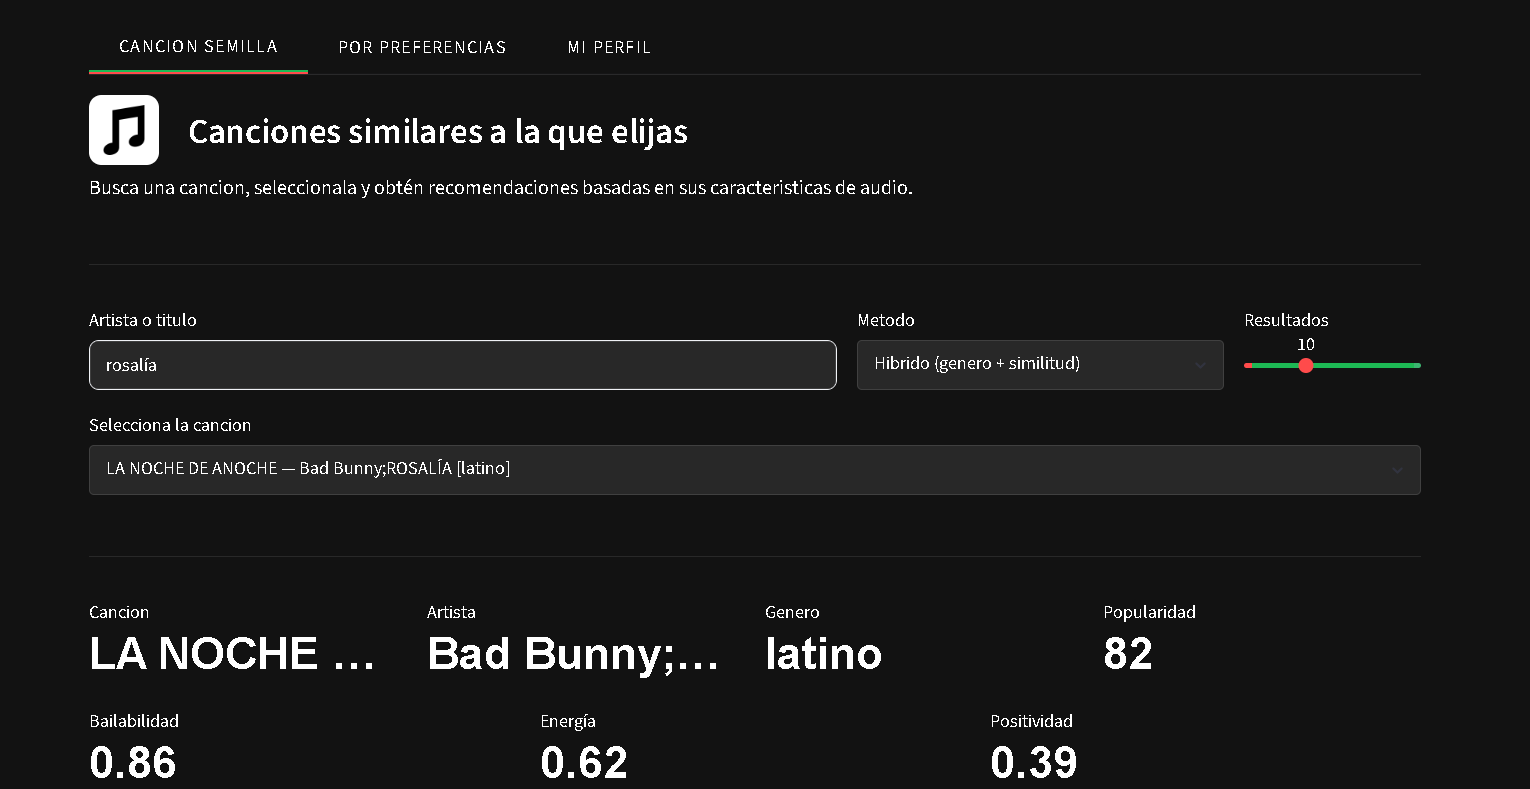
\includegraphics[width=\textwidth]{Captura_1}
  \caption{Interfaz de la aplicación web: pestaña ``Canción semilla''
           con la búsqueda de Bad Bunny y la selección de
           \textit{Tití Me Preguntó}. Se aprecian la barra de título
           personalizada, la paleta de color oscuro de Spotify,
           la información de la canción seleccionada y el botón
           de búsqueda de similares.}
  \label{fig:app_captura}
\end{figure}

\section{Síntesis y limitaciones de la aplicación}

La aplicación web cumple el objetivo de ofrecer los tres modos de
recomendación en una interfaz coherente, accesible y visualmente alineada
con la identidad de Spotify. Las principales limitaciones son:

\begin{itemize}
  \item \textbf{Sin persistencia en servidor}: el JSON de perfiles se
        almacena localmente. En un despliegue real, sería necesaria una
        base de datos compartida (p.ej.\ PostgreSQL o Redis).
  \item \textbf{Sin autenticación}: cualquier usuario puede acceder al
        perfil de otro si conoce su nombre. En producción se requeriría
        un sistema de autenticación.
  \item \textbf{Dataset estático}: el dataset no se actualiza
        automáticamente con nuevos lanzamientos de Spotify. Una versión
        más avanzada conectaría con la API de Spotify para enriquecer
        el catálogo en tiempo real.
  \item \textbf{Sin historial real}: los 8 perfiles sintéticos son una
        demostración; la calidad del recomendador mejora significativamente
        con historiales más largos (20--50 canciones), donde el perfil
        ponderado converge hacia una representación más estable del oyente.
\end{itemize}
